\documentclass[11pt,twoside,final
]{article}
\usepackage{amsmath,amsfonts,amssymb,amsthm,indentfirst,enumerate,textcomp}
\usepackage[utf8]{inputenc}
\usepackage{chebsb}
\usepackage[russian]{babel}
\usepackage{indentfirst, array}
\usepackage{amscd,latexsym}
\usepackage{mathrsfs}
%\usepackage[ruled, linesnumbered]{algorithm2e}
\usepackage{tabularx}
\usepackage{multirow}

\usepackage{graphicx}
\usepackage{textcase}% Оформление страниц

\graphicspath{ {./img/} }

\label{beg}
% заглавие стати и аннотация

\levkolonttl{%левый колонтитул - авторы
И.~Б.~Кожухов, А.~М.~Пряничников}
\prvkolonttl{%правый колонтитул - сокращенное название статьи
Об унарах с тождествами в решётке конгруэнций, II}

\newcommand{\god}{2025} % Для подавления ошибки при компиляции проекта

\UDK{% УДК статьи
512.567.5 + 512.579}

\DOI{
10.22405/2226-8383-\god-\tom-\iss-\pageref{beg}-\pageref{end}
}

\title
{%название статьи на русском языке с указанием источника финансирования при необходимости
Об унарах с тождествами в решётке конгруэнций, II}
{%название статьи на английском языке
On unars with identities in congruence lattice, II}

\author
{%авторы статьи
И. Б. Кожухов, А. М. Пряничников}
{%авторы статьи
I. B. Kozhukhov, A. M. Pryanichnikov}

\Cite{
И. Б. Кожухов, А. М. Пряничников. Об унарах с тождествами в решётке конгруэнций, II // Чебышевcкий сборник, \god, т.~\tom, вып.~\iss, с.~\pageref{beg}--\pageref{end}.
}
{Kozhukhov, I. B., Pryanichnikov, A. M. \god, ``On unars with identities in congruence lattice, II''\,, {\it Che\-by\-shev\-skii sbornik}, vol.~\tom, no.~\iss, pp.~\pageref{beg}--\pageref{end}.
}

\info
{%авторы статьи на русском языке
\noindent {\bf Кожухов Игорь Борисович}~--- д.ф.-м.н., Нац. исслед. университет МИЭТ; механико-математический факультет МГУ; Гос. академия нар. хоз-ва и гос. службы (г. Москва).

\noindent
\emph{e-mail: kozhuhov\_i\_b@mail.ru}

\noindent {\bf Пряничников Алексей Михайлович}~--- механико-математический факультет МГУ, ООО <<Квантом>> (г. Москва).

\noindent
\emph{e-mail: genary@ya.ru}


}
{%авторы статьи на английском языке
\noindent {\bf Kozhukhov Igor Borisovich}~--- Dr. Phys.-Math. Sci., Nat. Res. Univ. MIET; Fac. of Mech. and Math. of Moscow State Univ.; Russian Presidental Academy of Nat. Econom. and Public Admin., (Moscow).

\noindent
\emph{e-mail: kozhuhov\_i\_b@mail.ru}

\noindent {\bf Pryanichnikov Alexey Mikhailovich}~--- Fac. of Mech. and Math. of Moscow State Univ., <<Kvantom>> LLC, (Moscow).

\noindent
\emph{e-mail: genary@ya.ru}

}

\Abstract
{%Аннотация статьи на русском языке 150-250 слов с учетом ключевых слов
В статье доказано, что если решётка конгруэнций унара удовлетворяет нетривиальному решёточному тождеству, то унар является гомоморфным образом копроизведения конечного числа прямых и лучей.
}
{%Аннотация статьи на английском языке
In paper we prove that if a congruence lattice of an unar holds a nontrivial lattice identity, then the unar is a homomorphic image of the coproduct of finite number of lines and rays.
}

\keywords
{%ключевые слова на русском языке
полигон над полугруппой, унар, решётка конгруэнций, тождество.
}
{%ключевые слова на английском языке
act over semigroup, unar, congruence lattice, identity.
}

%число наименований в библиографии
\Bibliography{14 названий.}{14 titles.}

\def\Con{\operatorname{Con}}
\def\Eq{\operatorname{Eq}}
\def\indeg{\operatorname{indeg}}

\begin{document}

%генерация заглавия статьи
\maketitle

\enmaketitle

\section{Введение}

Решётка конгруэнций $\Con A$ универсальной алгебры $A$ — важная характеристика этой алгебры.
Это полная решётка с наименьшим элементом $\Delta = \{ (a,a) \mid a \in A \}$ и наибольшим элементом $\nabla = A \times A$, причём $\Con A$ является полной подрешёткой решётки $\Eq A$ всех отношений эквивалентности на множестве $A$.
Изучение алгебр с условиями на решётку конгруэнций — активно развивающееся и богатое содержанием направление общей алгебры.
Сюда относятся условия максимальности и минимальности, приводящие к понятиям артиновых и нётеровых алгебр, условие простоты (когда $\Con A = \{ \Delta, \nabla \}$), антипростоты ($\Con A = \Eq A$), дистрибутивности или модулярности (т.е. решётка $\Con A$ дистрибутивна или модулярна), подпрямой неразложимости и т.д.

Алгебрам $A$, у которых решётка конгруэнций $\Con A$ является дистрибутивной или модулярной, посвящено значительное число работ разных авторов.
Дистрибутивные и модулярные полигоны над полугруппами изучались в~\cite{Ptakhov_2}, полное описание таких полигонов над полугруппами левых или правых нулей получено в~\cite{Khaliullina_3}.
В работе~\cite{Egorova_4} были описаны дистрибутивные и модулярные унары.
Дистрибутивность решётки $\Con A$ означает выполнение в ней тождества $ (x \vee y) \wedge z = (x \wedge z) \vee (y \wedge z) $, модулярность задаётся тождеством $ (x \vee y) \wedge (x \vee z) = x \vee (z \wedge (x \vee y)) $.
Естественным представляется изучение алгебр $A$, у которых решётка $\Con A$ удовлетворяет какому-нибудь нетривиальному решёточному тождеству.
Данное условие является \textit{условием конечности}, так как любая конечная алгебра ему удовлетворяет (это следует из того, что всякая конечная решётка удовлетворяет нетривиальному тождеству — см. лемму~\ref{lemma:3}).
Многообразия алгебр, у которых решётки конгруэнций всех алгебр удовлетворяют одному и тому же нетривиальному тождеству, посвящены монография~\cite{Kearnes_5} и диссертация~\cite{Nation_6}.
В работе~\cite{Repnitsky_7} были описаны коммутативные полугруппы, у которых решётки подполугрупп удовлетворяют нетривиальному решёточному тождеству.
Цель данной работы — найти необходимое условие того, что решётка конгруэнций унара (полигона над свободной циклической полугруппой) удовлетворяет нетривиальному тождеству.
Является ли это условие достаточным, авторам неизвестно.

Работа является продолжением работы~\cite{Kozhukhov_8}, поэтому за доказательствами некоторых утверждений мы будем отсылать читателя к этой работе.
Отметим, что заключительное утверждение, сформулированное в последнем абзаце работы~\cite{Kozhukhov_8}, требует корректировки: вместо «копроизведения конечного числа прямых» следовало написать «копроизведения конечного числа прямых и лучей».

Основные сведения из универсальной алгебры можно найти в~\cite{Kohn_9}, из теории решёток — в~\cite{Gretzer_10}, теории полугрупп — в~\cite{Clifford_11}, полигонов над полугруппами — в~\cite{Kilp_1}, унаров — в~\cite{Jakubikova_12}, многообразий решёток — в~\cite{Jipsen_13}.

\section{Основные определения}

\textit{Полигон над полугруппой} — это множество $X$, на котором действует полугруппа $S$, т.е. определено отображение $X \times S \to X$, $(x,s) \mapsto xs$ удовлетворяющее условию $x(st) = (xs)t$ при $x \in X$, $s,t \in S$ (см.~\cite{Kilp_1}).
Полигон над полугруппой является алгебраической моделью \textit{автомата}.
Кроме того, понятие полигона фактически совпадает с понятием \textit{унарной алгебры}.

Подмножество $Y \subseteq X$ называется \textit{подполигоном}, если $YS \subseteq Y$.
Элемент $z \in X$ называется \textit{нулём}, если $zs = z$ при всех $s \in S$.
Нулей у полигона, в отличие от полугруппы, может быть сколько угодно (в полугруппе нуль, если он существует, единственен).
\textit{Решётку конгруэнций} полигона $X$ над полугруппой $S$ мы будем обозначать $\Con_S X$ или просто $\Con X$.

Пусть $X$ — полигон над полугруппой $S$ и $Y$ — его подполигон.
Положим $ \rho_Y = (Y \times Y) \cup \Delta_X $.
Это конгруэнция полигона $X$, называемая \textit{конгруэнцией Риса}, соответствующей подполигону $Y$.
Нетрудно видеть, что для любого подполигона $Y$, у конгруэнции Риса $\rho_Y$ один из классов есть множество $Y$, а другие классы одноэлементны.
Для фактор-полигона $X/\rho_Y$ мы будем также использовать краткую запись: $X/Y$.

Пусть $X$ — полигон над полугруппой $S$ и $X_i$ ($i \in I$) — его подполигоны, причём $X = \bigcup_{i \in I} X_{i}$ и $X_{i} \cap X_{j} = \varnothing$ при $i \neq j$.
В этом случае мы называем полигон $X$ \textit{копроизведением} полигонов $X_i$ и пишем $X = \bigsqcup_{i \in I} X_{i}$.
В работах по унарам копроизведение называют обычно прямой суммой.

Для полугруппы $S$ полагаем $S^1 = S \cup \{ 1 \}$.
Здесь $S^1$ — полугруппа, полученная присоединением к $S$ внешним образом единицы (при этом считаем, что $s \cdot 1 = 1 \cdot s = s$ для каждого $s \in S^1$).
Если $X$ — полигон над $S$, то его можно сделать полигоном над полугруппой $S^1$, положив $x \cdot 1 = x$ при $x \in X$.

\textit{Унар}, т.е. множество $X$ с одной унарной операцией $f: X \to X$, мы здесь будем рассматривать как полигон над свободной циклической полугруппой $S = \{ a,a^{2},a^{3},\ldots\}$, при этом $x \cdot a = f(x)$, $x \cdot a^i = f^i (x)$ при $i \geqslant 1$, $f^0(x) = x$ для всех $x \in X$.
Унар $X$ называется \textit{связным}, если для любых $x,y \in X$ существуют такие $k,l \geqslant 0$, что $x a^k = y a^l$.
Нетрудно видеть, что любой унар является копроизведением связных подунаров $X_i$ (\textit{компонент связности}).
Для унара $X$ и элемента $x \in X$ полагаем $xS = \{ xa^k \mid k \geqslant 1 \}$, $xS^{-1} = \{ y \mid \exists k \geqslant 1 \ y a^k = x \}$, $xa^{-1} = \{ y \mid ya = x \}$.

Приведём также некоторые определения из теории графов.
В ориентированном графе $G$ с множеством вершин $V(G)$ и рёбер $E(G)$ для каждой вершины $x \in V(G)$ определяются понятия \textit{входной степени}
\[
	\indeg x = |\{ y \mid (y,x) \in E(G) \}|
\]
вершины $x$.
Понятно, что у унара $X$, рассматриваемого как граф, $\indeg x = |xa^{-1}|$ для всех $x \in X$.

Пусть $X$ -- унар.
Элемент $x \in X$ назовём \textit{узлом}, если существуют элементы $y,z \in X$ такие, что $y \neq z$ и $y \cdot a = z \cdot a = x$.
Приведённое здесь определение узла отличается от определения в~\cite{Kozhukhov_8}.
Элементы $x \in X \setminus XS$ будем называть \textit{начальными}.
Эквивалентное определение: элемент $x$ унара $X$ называется \textit{начальным}, если не существует такого элемента $y \in X$, что $ya = x$.
Элемент $x \in X$ \textit{периодический}, если $x \cdot a^n = x$ для некоторого $n > 0$.

На полигоне $X$ над полугруппой $S$ можно ввести отношение \textit{квазипорядка} $\leqslant$ (рефлексивное и транзитивное отношение), полагая $x \leqslant y \Leftrightarrow x \in y S^1$.

\textit{Циклом} $C_n = \{ c_0, c_1, \ldots, c_{n - 1} \}$ длины $n$ называется унар, изоморфный унару $\mathbb{Z}_n = \{ 0, 1, \ldots, n - 1 \}$ с операцией $i \cdot a = i + 1 \ (\textrm{mod } n)$ (см. рисунок~\ref{fig:line_ray_cycle}, справа).
\textit{Хвостом} цикла $C$ называется неодноэлементное подмножество унара $X$, являющееся цепью относительно отношения $\leqslant$ с наименьшим элементом $c \in C$, который будем называть \textit{входом} хвоста.
\textit{Длиной} хвоста назовём число элементов хвоста, не принадлежащих циклу.
В данной работе мы будем рассматривать только простые циклы (см. рисунок~\ref{fig:line_ray_cycle}, справа), либо циклы с конечными либо бесконечными хвостами (см. рисунок~\ref{fig:tails}).
\begin{figure}[ht!]
	\centering
	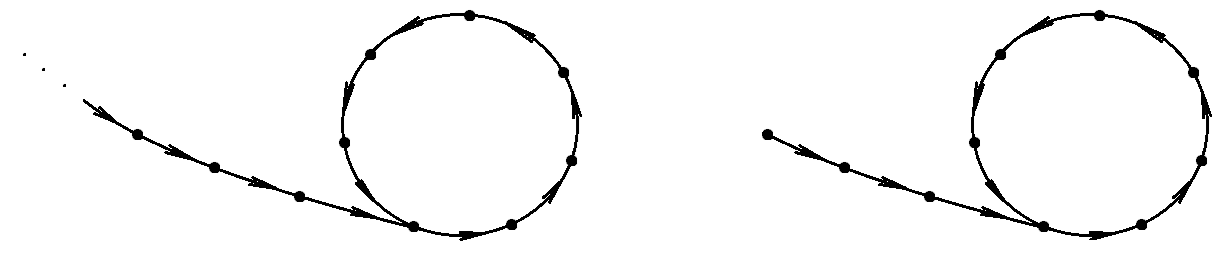
\includegraphics[scale=0.4]{img/tails.png}
	\caption{Цикл с бесконечным хвостом (слева) и с конечным хвостом (справа).}
	\label{fig:tails}
\end{figure}
\textit{Прямой} называется унар, изоморфный унару $\mathbb{Z}$ с операцией $i \cdot a = i + 1$ при $i \in \mathbb{Z}$ (см. рисунок~\ref{fig:line_ray_cycle}, слева).
Также прямой можно считать цикл бесконечной длины либо унар, являющийся цепью относительно $\leqslant$.
\textit{Лучом} называется унар, изоморфный унару $\mathbb{N}$ с операцией $i \cdot a = i + 1$ при $i \in \mathbb{N}$ (см. рисунок~\ref{fig:line_ray_cycle}, по центру).
\begin{figure}[ht!]
	\centering
	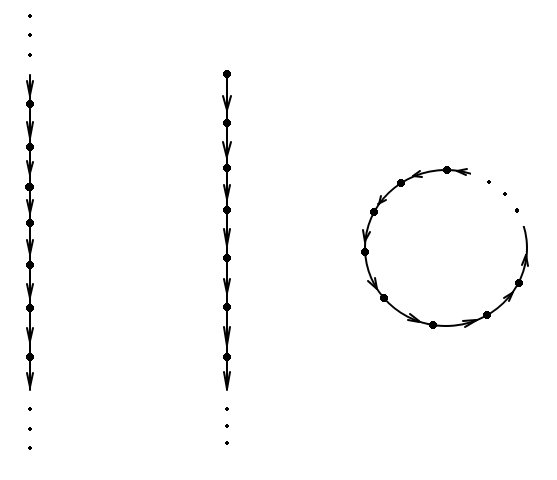
\includegraphics[scale=0.5]{img/line_ray_cycle.png}
	\caption{Прямая (слева), луч (по центру) и цикл (справа).}
	\label{fig:line_ray_cycle}
\end{figure}
Нетрудно увидеть, что унары, не содержащие узлов, -- это в точности прямые, лучи либо циклы, изображённые на рисунке~\ref{fig:line_ray_cycle}.

\begin{lemma}[{\cite[лемма 1]{Kozhukhov_8}}] \label{lemma:1}
	Если $X$ — полигон над полугруппой $S$, $Y$ — его подполигон и $\rho_Y$ — конгруэнция Риса, то решётки $\Con Y$ и $\Con (X/Y)$ изоморфно вкладываются в решётку $\Con X$.
\end{lemma}

Для дальнейшего нам понадобится несколько фактов из теории многообразий решёток.
Решётка $L$ называется \textit{нетривиальной}, если $|L| > 1$.
Решёточное тождество $p \approx q$ называется \textit{нетривиальным}, если оно выполняется не во всех решётках, но выполняется в какой-либо нетривиальной решётке.
Здесь $p,q$ — термы сигнатуры $\{ \land , \lor \}$.

\begin{lemma}\label{lemma:2}
	Решётка $\Eq A$, где $A$ -- бесконечное множество, не удовлетворяет никакому нетривиальному тождеству.
\end{lemma}
\begin{proof}
	По~\cite[предпоследнее следствие]{Sachs_14} не существует нетривиального тождества, выполняющегося в любой решётке $\Eq A$, где $A$ -- бесконечное множество.
	Так как тривиальные тождества выполняются во всех решётках, то в $\Eq A$ выполняются только они.
\end{proof}

Следующее утверждение известно, его доказательство можно получить на основании~\cite[следствие 3.14]{Kohn_9} и~\cite[теорема 8 главы VI]{en_Gretzer_10} (см. также~\cite[лемма 3]{Kozhukhov_8}).
\begin{lemma}\label{lemma:3}
	Всякая конечная решётка удовлетворяет некоторому нетривиальному тождеству.
\end{lemma}

\begin{lemma}[{\cite[леммы 4,5,6]{Kozhukhov_8}}] \label{lemma:4}
	Пусть $X$ — унар.
	Если решётка $\Con X$ удовлетворяет нетривиальному тождеству, то:
	\begin{enumerate}
		\item $X$ имеет лишь конечное число компонент связности;
		\item множество $X \setminus XS$ конечно (т.е. количество начальных элементов конечно);
		\item $X$ имеет лишь конечное число периодических элементов;
		\item $X$ не содержит бесконечного множества попарно несравнимых относительно естественного квазипорядка ($\leqslant$) элементов.
	\end{enumerate}
\end{lemma}

Следует отметить, что в доказательстве~\cite[лемма 4(2)]{Kozhukhov_8} имеется ошибка, а именно, утверждается, что фактор-полигон $X / XS$ состоит из нулей.
Это неверно. Однако, $X / XS$ является полигоном с нулевым умножением, а значит, $\Con (X/XS) = \Eq (X/XS)$, что делает верным доказательство леммы.

\section{Предварительные результаты}

Приведём вспомогательные леммы, необходимые для доказательства основных результатов работы.
\begin{lemma} \label{lemma:5}
	Если решётка $\Con X$ унара $X$ удовлетворяет нетривиальному тождеству, то $\indeg x < \infty$ для каждого $x \in X$.
\end{lemma}
\begin{proof}
	Предположим, что утверждение леммы неверно, т.е. множество $xa^{-1}$ бесконечно при некотором $x \in X$.
	Отсюда следует, что можно найти различные элементы $y_1, y_2, \ldots \in X $ такие, что $y_n a = x$ при всех $n \in \mathbb{N}$.
	Рассмотрим унар $Y = \bigcup_{n \in \mathbb{N}} y_n S$ и фактор-унар $\overline{Y} = Y / x S^1$.
	Так как решётка $\Con X$ удовлетворяет нетривиальному тождеству, то по лемме~\ref{lemma:1} решётка $\Con \overline{Y}$ удовлетворяет тому же тождеству.
	Но это невозможно, так как унар $Y$ является унаром с нулевым умножением, а значит, $\Con \overline{Y} = \Eq \overline{Y}$, что противоречит лемме~\ref{lemma:2} ввиду того, что множество $\overline{Y}$ бесконечно.
\end{proof}

\begin{lemma} \label{lemma:6}
	Если решётка $\Con X$ унара $X$ удовлетворяет нетривиальному тождеству, то $X$ имеет лишь конечное число узлов.
\end{lemma}
\begin{proof}
	Нетрудно увидеть, что все узлы делятся на два типа (см. рисунок~\ref{fig:uzly_1}): где $x \notin \{ y, z \}$ и где $x \in \{ y, z \}$.
	\begin{figure}[ht!]
		\centering
		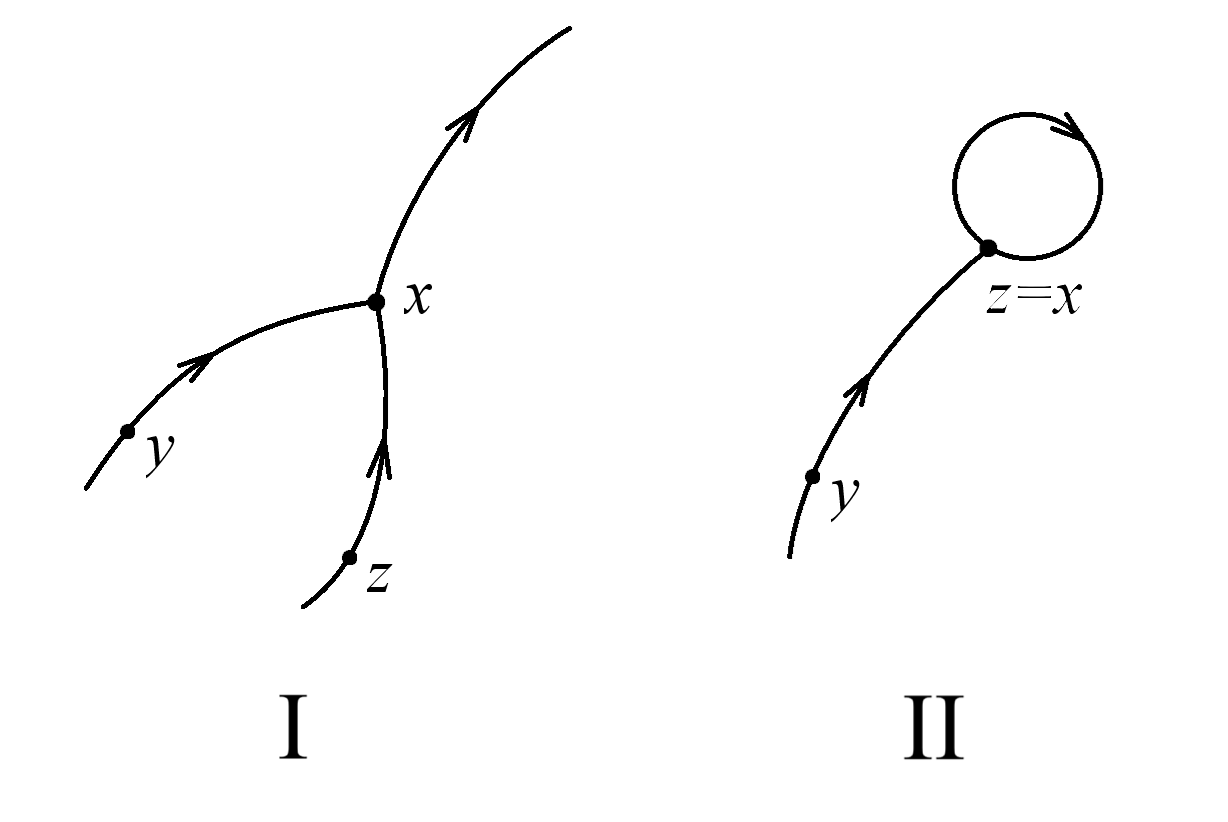
\includegraphics[scale=0.4]{img/uzly_1.png}
		\caption{Типы узлов.}
		\label{fig:uzly_1}
	\end{figure}
	Очевидно, что узлов второго типа в одной компоненте связности может быть не более одного (см. лемму~\ref{lemma:4}(3)).
	Так как по лемме~\ref{lemma:4}(1) компонент связности конечное число, то и число таких узлов тоже конечно.

	Осталось показать, что узлов первого типа конечное число.
	Пусть это не так, т.е. их бесконечно много.
	Так как по лемме~\ref{lemma:4}(1) число компонент связности конечно, то узлов первого типа бесконечно много в какой-либо компоненте.
	Рассмотрим эту компоненту связности, обозначим её через $Y$, возьмём в ней какой-нибудь узел $u_0$ и разберём два случая.

	\textit{Случай 1}: среди элементов $u_0 a, u_0 a^2, u_0 a^3, \ldots$ бесконечно много узлов.
	Тогда $u_0, u_0 a^{i_1}, u_0 a^{i_2}, \ldots$ -- узлы, где $0 < i_1 < i_2 < \ldots$.
	Положим $u_k = u_0 a^{i_k}$ $(k=1,2,\ldots)$.
	Так как $u_k$ -- узел, то существует $v_k \neq u_0 a^{i_k - 1}$ такое, что $v_k a = u_k$ (см. рисунок~\ref{fig:uzly_2}).
	\begin{figure}[ht!]
		\centering
		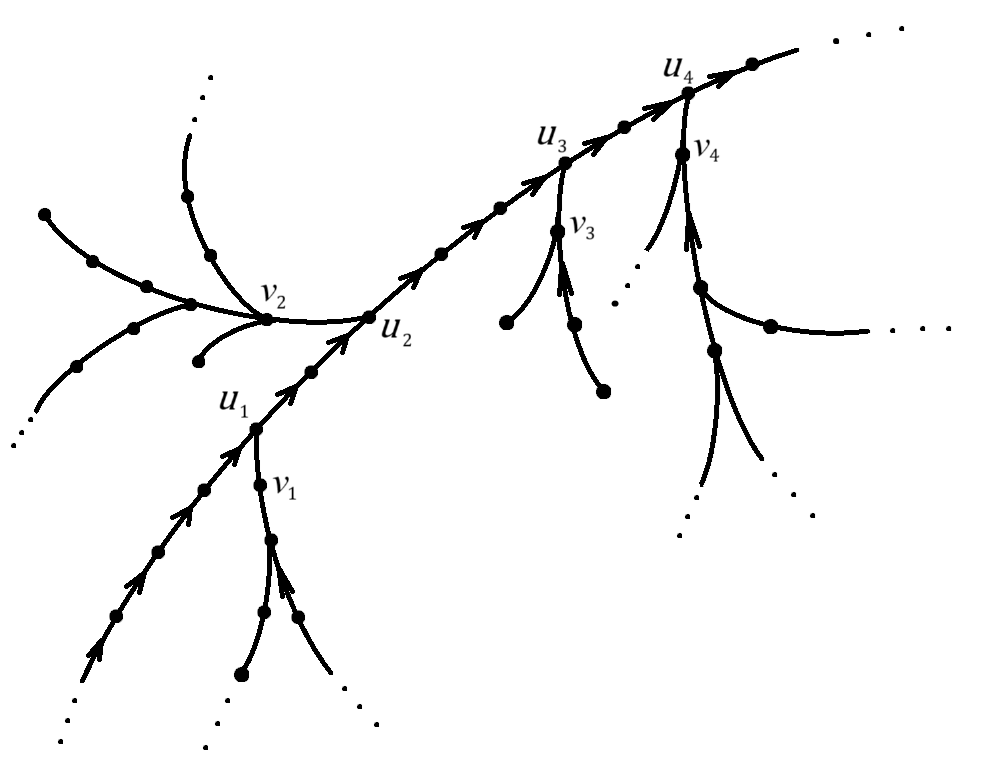
\includegraphics[scale=0.5]{img/uzly_2.png}
		\caption{Узлы $u_0, u_1, u_2, \ldots$.}
		\label{fig:uzly_2}
	\end{figure}
	Так как подунар $u_0 S^1$ бесконечен, то $v_k \notin u_0 S^1$.
	Пусть $\overline{Y} = Y / u_0 S^1$ и обозначим через $z$ нуль этого унара (см. рисунок~\ref{fig:uzly_3}).
	\begin{figure}[ht!]
		\centering
		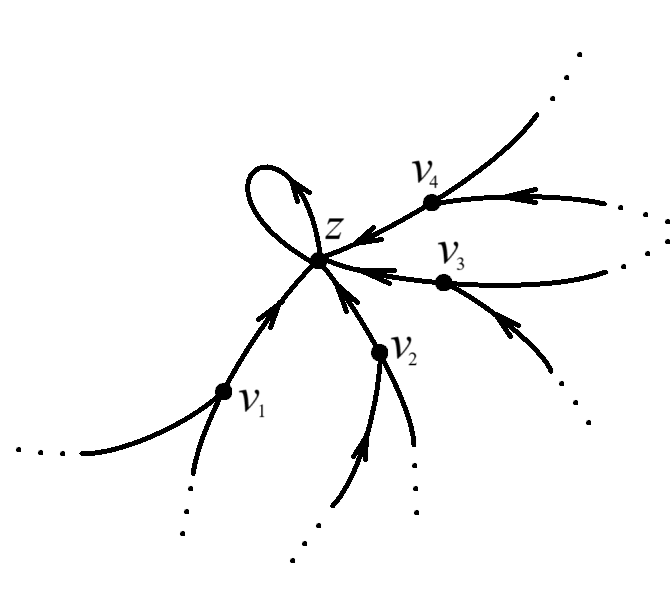
\includegraphics[scale=0.6]{img/uzly_3.png}
		\caption{Фактор-унар $\overline{Y} = Y / u_0 S^1$.}
		\label{fig:uzly_3}
	\end{figure}
	Очевидно, элементов $v_1, v_2, \ldots$ бесконечное число, все они различны в унаре $\overline{Y}$, поэтому $\indeg z = \infty$, что противоречит лемме~\ref{lemma:5}.

	\textit{Случай 2}: среди элементов $u_0 a,u_0 a^{2},u_0 a^{3},\ldots$ лишь конечное число узлов унара $X$.
	Здесь возможны две ситуации: либо последовательность $u_0, u_0 a, u_0 a^2, \ldots$ заканчивается циклом длины $m$: $\{ u_0 a^r, u_0 a^{r + 1}, \ldots, u_0 a^{r + m - 1} \}$ $(u_0 a^{r + m} = u_0 a^r)$, либо элементы $u_0, u_0 a, u_0 a^2, \ldots$ различны, и тогда есть последний узел $u_0 a^k$, т.е. такой узел, что элементы $u_0 a^t$ при $t > k$ не являются узлами.
	И в той, и в другой ситуации мы имеем, что все узлы унара $Y$ лежат в множестве $\{ y_0 \} \cup y_0 S^{-1}$ для некоторого $y_0 \in Y$, который можно считать узлом.
	По лемме~\ref{lemma:5} множество $y_0 a^{-1}$ конечно.
	Пусть $y_0 a^{-1} = \{ x_1, \ldots, x_m \}$.
	Очевидно, в каком-либо из множеств $x_i S^{-1}$ лежит бесконечно много узлов.
	Можно считать, что множество $x_1 S^{-1}$ содержит бесконечно много узлов.
	Если $x_1$ -- узел, то положим $y_1 = x_1$ и перейдём к множеству $y_1 a^{-1}$, поступая с ним так же, как с множеством $y_0 a^{-1}$.
	Если же $x_1$ -- не узел, то множество $x_1 a^{-1}$ состоит из одного элемента.
	Так как $x_1 S^{-1} = \{ x_1 \} \cup x_1 a^{-1} \cup x_1 a^{-1} S^{-1} $ и $x_1 S^{-1}$ содержит бесконечно много узлов, то при каком-то $t$ мы получим узел $x_1 a^{-t}$, причём можно считать, что элементы $x_1, x_1 a^{-1}, \ldots, x_1 a^{-(t-1)}$ не являются узлами.
	Положим $y_1 = x_1 a^{-t}$ и поступим с элементом $y_1$ так же, как поступили с элементом $y_0$.
	Продолжая этот процесс, мы получим узлы $y_1,y_2,\ldots$ такие, что $y_k a^{j_k} = y_{k - 1}$ при подходящих $j_k > 0$ $(k = 1,2,\ldots)$.
	Так как $y_k$ -- узлы, то существуют $z_k \in Y$ такие, что $z_k a = y_k$ и $z_k \notin y_{k + 1}S$ (см. рисунок~\ref{fig:uzly_4}).
	Очевидно, что так как узлов $y_k$ бесконечно много, то и элементов $z_k$ тоже.
	\begin{figure}[ht!]
		\centering
		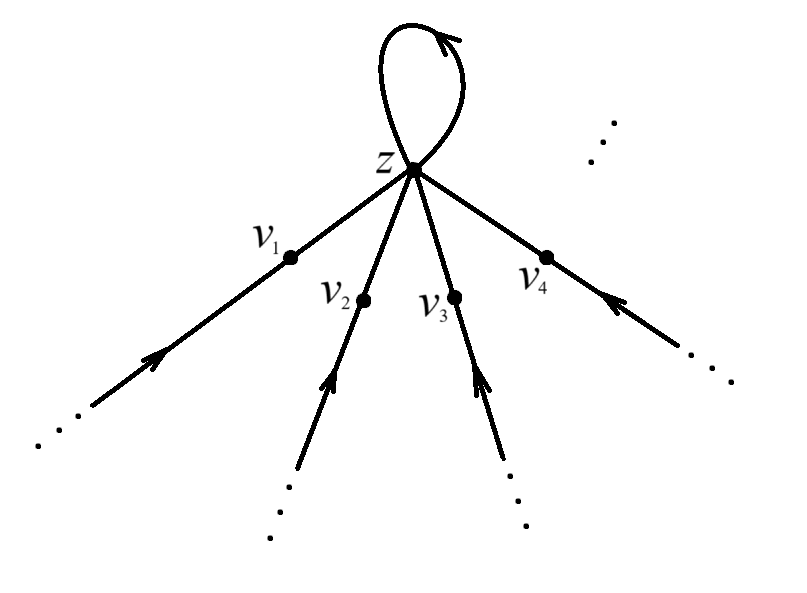
\includegraphics[scale=0.45]{img/uzly_4.png}
		\caption{Узлы $y_0, y_1, y_2, \ldots$.}
		\label{fig:uzly_4}
	\end{figure}
	Пусть $Y' = \bigcup_{k=1}^{\infty} y_k S$ и $\overline{Y} = Y / Y'$.
	По лемме~\ref{lemma:1} решётка $\Con \overline{Y}$ удовлетворяет нетривиальному тождеству.
	Однако, в унаре $\overline{Y}$ выполняется равенство $z_k a = 0$ при всех $k \in \mathbb{N}$, где $0$ обозначает нулевой элемент унара $\overline{Y}$.
	Поэтому $\indeg 0 = \infty$, а это противоречит лемме~\ref{lemma:5}.
\end{proof}

\section{Основные результаты}

Теперь мы можем привести первый из основных результатов нашей работы.
\begin{theorem} \label{thm:main_1}
	Если $X$ -- унар, у которого решётка конгруэнций $\Con X$ удовлетворяет нетривиальному решёточному тождеству, то $X$ удовлетворяет условиям:
	\begin{enumerate}
		\item[(i)] $X$ имеет лишь конечное число компонент связности;
		\item[(ii)] $X$ имеет лишь конечное число начальных элементов;
		\item[(iii)] $X$ имеет лишь конечное число узлов;
		\item[(iv)] $\indeg x < \infty$ для каждого $x \in X$.
	\end{enumerate}
\end{theorem}
\begin{proof}
	Утверждение \textit{(i)} следует из леммы~\ref{lemma:4}(1), \textit{(ii)} -- из леммы~\ref{lemma:4}(2), \textit{(iii)} -- из леммы~\ref{lemma:6}, \textit{(iv)} -- из леммы~\ref{lemma:5}.
\end{proof}
Авторам неизвестно, верно ли утверждение, обратное к теореме~\ref{thm:main_1}, т.е. следует ли из условий \textit{(i)--(iv)} выполнение нетривиального тождества в решётке $\Con X$.
В работе~\cite{Egorova_4} для некоторых унаров, удовлетворяющих \textit{(i)--(iv)}, доказана дистрибутивность или модулярность решётки $\Con X$.

Выясним теперь строение унаров, удовлетворяющих условиям \textit{(i)-(iv)} только что доказанной теоремы.
Следующая лемма является несложным упражнением по теории полигонов.
\begin{lemma} \label{lemma:7}
	Пусть $X$ -- полигон над полугруппой $S$ такой, что $X = \bigcup_{i \in I} X_i$, где $X_i$ -- подполигоны.
	Тогда $X$ является гомоморфным образом копроизведения $X' = \coprod_{i \in I} X_i$.
\end{lemma}
\begin{proof}
	Отображение $\pi: X' \rightarrow X$, $x \mapsto x$ является гомоморфизмом таким, что $\pi(X') = X$.
\end{proof}

Вторым из основных результатов работы является следующая теорема.
\begin{theorem} \label{thm:main_2}
	Унар $X$ удовлетворяет условиям \textit{(i)-(iv)}, сформулированным в теореме~\ref{thm:main_1}, в том и только том случае, если $X$ является гомоморфным образом копроизведения конечного числа прямых и лучей.
\end{theorem}
\begin{proof}
	\textit{Необходимость.}
	Пусть выполняются условия \textit{(i)-(iv)}.
	Для начала введём обозначения подунаров $K_i$, $V_i$ и $U_{ij}$.
	Выделим компоненты связности унара $X$, являющимися прямыми, лучами или циклами.
	По условию \textit{(i)} их конечное число, обозначим из через $K_1, K_2, \ldots, K_r$.
	Это компоненты связности без узлов, а значит, остальные компоненты имеют узлы.

	По условию \textit{(ii)} начальных элементов лишь конечное число, обозначим их через $v_1,\ldots, v_n$.
	Для каждого начального элемента пусть $V_i = v_i S^1$, $(i=1,2,\ldots,n)$.
	Очевидно, $V_i$ -- луч или цикл с конечным хвостом.

	Если $x \in X$ -- элемент унара, то выберем произвольный $x' \in x a^{-1}$, затем $x'' \in x' a^{-1}$ и т.д.
	Полученную последовательность обозначим через $M(x) = \{x, x', x'', \ldots \}$.

	Перейдём теперь к узлам.
	По условию \textit{(iii)} их конечное число, обозначим их через $u_1, \ldots, u_m$.
	Для произвольного узла $u_i$ опеределим подунар $U_{ij}$ следующим образом.
	Так как из условия \textit{(iv)} следует, что множество $u_i a^{-1}$ конечно, то пусть $u_i a^{-1} = \{ x_1, \ldots, x_{t_i} \}$.
	Возьмём какой-либо $x_j \in u_i a^{-1}$ и положим:
	\[
		U_{ij} =
		\begin{cases}
			u_i S^1,             & \text{если } M(x_j) \text{ содержит начальный элемент либо узел};    \\
			u_i S^1 \cup M(x_j), & \text{если } M(x_j) \text{ не содержит узлов и начальных элементов}.
		\end{cases}
	\]
	Ясно, что тогда $U_{ij}$ -- прямая или цикл с бесконечным хвостом.

	Теперь докажем, что
	\[
		X = \bigcup_{i = 1}^r K_i \cup \bigcup_{i = 1}^n V_i \cup \bigcup_{i = 1}^m \bigcup_{j = 1}^{t_i} U_{ij}.
	\]
	Пусть $x \in X$ -- произвольный элемент.
	Если $x$ лежит в компоненте связности без узлов, то $x \in \bigcup_{i = 1}^r K_i$;
	Пусть $x$ лежит в компоненте связности с узлами.
	Если $x$ -- узел, то $x \in U_{ij}$ при некоторых $i,j$.
	Далее считаем, что $x$ -- не узел, но лежит в компоненте связности с узлами.
	Рассмотрим последовательность $M(x)$.
	% Положим $x^{(0)} = x$ и будем строить последовательность $x^{(1)}, x^{(2)}, \ldots$, как показано выше, т.е. пока множество $x^{(k)} a^{-1}$ одноэлементно.
	Если в этой последовательности какие-либо элементы совпадут друг с другом, то $x^{(k)} = x$ при некотором $k$.
	Следовательно, $x$ лежит в цикле, в котором нет ни одного узла унара $X$.
	Тогда $x \in \bigcup_{i = 1}^r K_i$, а это противоречит требованию к элементу $x$.
	Если в этой последовательности окажется начальный элемент, то $x \in V_i$ при некотором $i$.
	Если в этой последовательности окажется узел $u_k$, то $x \in U_{km}$ для некоторого $m$.
	Пусть теперь элементы $x^{(0)}, x^{(1)}, x^{(2)}, \ldots$ различны.
	Тогда рассмотрим элементы $xa, xa^2, xa^3, \ldots$.
	Если ни один из элементов $xa, xa^2, \ldots$ не является узлом, то $x$ лежит в компоненте связности, являющейся прямой, т.е. $x \in \bigcup_{i = 1}^r K_i$, что противоречит требованию к $x$.
	Если какой-либо элемент из множества $xS$ является узлом, то $x a^k = u_i$ при некоторых $i,k$.
	Легко видеть, что тогда $x \in U_{ij}$ при некоторых $i,j$.
	Если какие-либо из элементов $x^{(0)}, x^{(1)}, x^{(2)}, \ldots$ совпадают, то мы имеем либо цикл без узлов, либо цикл с хвостом.
	В случае, если $x \in C_n$, то $x \in \bigcup_{i = 1}^r K_i$, т.е. получаем противоречие.
	В случае, если у нас цикл с хвостом, то существует узел $u_i \in xS$ и $x \in U_{ik}$ при некоторых $i,k$.

	Так как $K_i$, $V_i$ и $U_{ij}$ -- подунары унара $X$, то обратное включение очевидно.
	Заметим, что гомоморфный образ прямой -- это прямая, или цикл, или цикл с бесконечным хвостом, а гомоморфный образ луча -- луч, или цикл, или цикл с конечным хвостом.
	Из этого, а также из леммы~\ref{lemma:7} следует, что $X$ является гомоморфным образом копроизведения конечного числа прямых и лучей.

	\textit{Достаточность}.
	Пусть $X = \varphi(\coprod_{i = 1}^{n} L_i)$, где $\varphi: \coprod_{i = 1}^{n} L_i \rightarrow X$ -- сюръективный гомоморфизм, $L_i$ -- прямая либо луч.
	Пусть $c(X)$ -- мощность множества компонент связности, $b(X)$ -- множества начальных элементов, $k(X)$ -- множества узлов унара $X$.
	Так как при гомоморфизме число компонент связности увеличиться не может, то $c(X) \leqslant n$.
	Далее, нетрудно увидеть, что при гомоморфизме элемент, не являющийся начальным, не может перейти в начальный, поэтому $b(X)$ не превышает количества лучей среди $L_i$, а следовательно, $b(x) \leqslant n$.

	Нетрудно увидеть, что унар можно представить как объединение подунаров (возможно, пересекающихся), являющихся прямыми, лучами либо циклами (с хвостами либо без).
	% Это можно увидеть, взяв любой $x \in X$ и подымаясь наверх и вниз.

	% Узел в $X$ может образоваться лишь склейкой элементов одной прямой либо луча, либо элементов множества различных прямых либо лучей, а раз их число конечно, то $k(X) \leqslant n$.
	% Наконец, очевидно, что если бы $\indeg x = \infty$ для некоторого узла $x$, то он может получиться только склейкой бесконечного числа прямых либо лучей, что невозможно.
\end{proof}

\section{Заключение}

Доказано, что ...

\begin{corollary}
	Если решётка конгруэнций $\Con X$ унара $X$ удовлетворяет нетривиальному решёточному тождеству, то $X$ является гомоморфным образом копроизведения конечного числа прямых и лучей.
\end{corollary}
\begin{proof}
	Следует из теорем~\ref{thm:main_1} и~\ref{thm:main_2}.
\end{proof}

%библиография по ГОСТу
\begin{thebibliography}{99}

	\bibitem{Kilp_1}
	Kilp~M., Knauer~U., Mikhalev~A.\,V. Monoids, acts and categories // Berlin - N.Y., de Gruyter, 2000. 529 P.

	\bibitem{Ptakhov_2}
	Птахов~Д.\,О., Степанова~А.\,А. Решётки конгруэнций полигонов // Дальневост. матем. журн. 2013. Т.~13, №1. С.~107--115.

	\bibitem{Khaliullina_3}
	Халиуллина~А.\,Р. Условия модулярности решётки конгруэнций полигона над полугруппой правых или левых нулей // Дальневост. матем. журн. 2015. Т.~15, №~1. С.~102--120.

	\bibitem{Egorova_4}
	Егорова~Д.\,П. Структура конгруэнций унарной алгебры // Межвузовский научный сборник «Упорядоченные множества и решётки». г. Саратов: Издательство Саратовского университа. 1978. Вып.~5. С.~11--43.

	\bibitem{Kearnes_5}
	Kearnes~K.\,A., Kiss~E.\,W. The shape of congruence lattices // Memoirs of the American Mathematical Society. 2013. Vol.~222. 169 P.

	\bibitem{Nation_6}
	Nation~J.\,B. Varieties of algebras whose congruence lattices satisfy lattice identities (Thesis) // Pasadena: California Institute of Technology. 1973. 63 P.

	\bibitem{Repnitsky_7}
	Репницкий~В.\,Б., Кацман~С.\,И. Коммутативные полугруппы, решётка подполугрупп которых удовлетворяет нетривиальному тождеству // Математический сборник. 1988. Т.~137(179), №~4(12). С.~462--482.

	\bibitem{Kozhukhov_8}
	Кожухов~И.\,Б., Пряничников~А.\,М. Об унарах с тождествами в решётке конгруэнций // Материалы VI международной научно-технической конференции СИТОНИ-2019. Донецк, 2019. С.~64--69.

	\bibitem{Kohn_9}
	Кон~П.\,М. Универсальная алгебра // М.: Мир, 1968. 359~С.

	\bibitem{Gretzer_10}
	Гретцер~Г. Общая теория решёток // М.: Мир, 1982. 454~С.

	\bibitem{Clifford_11}
	Клиффорд~А., Престон~Г. Алгебраическая теория полугрупп // М.: Мир, 1972. Т.~1. 286~с.; Т.~2. 423~С.

	\bibitem{Jakubikova_12}
	Jakubiková-Studenovská~D., Pócs~J. Monounary algebras // Košice: UPJS, 2009. 301~P.

	\bibitem{Jipsen_13}
	Jipsen~P., Rose~H. Variety of lattices // Lecture Notes in Mathematics, 1992. Vol.~1533. 166~P.

	\bibitem{Sachs_14}
	Sachs D. Identities in finite partition lattices // Proc. Amer. Math. Soc., 1961. Vol.~12. Iss.~6, PP.~944--945.

\end{thebibliography}


%библиография по Гарвардскому стандарту
\begin{engbibliography}{99}

	\bibitem{en_Kilp_1}
	Kilp, M., Knauer, U. \& Mikhalev, A.\,V. 2000, ``Monoids, acts and categories``, \textit{Berlin; New York: de Gruyter}, 546 pp.

	\bibitem{en_Ptakhov_2}
	Ptahov, D.\,O. Stepanova, A.\,A. 2013, ``Congruence lattice of S-acts``, \textit{Far Eastern Mathematical Journal}, vol. 13, no. 1, pp. 107--115.

	\bibitem{en_Khaliullina_3}
	Khaliullina, A.R. 2015, ``Modularity conditions of the lattice of congruences of acts over right or left zero semigroups``, \textit{Far Eastern Mathematical Journal}, vol. 15, no. 1, pp. 102--120.

	\bibitem{en_Egorova_4}
	Egorova, D.\,P. 1978, ``The structure of congruences of unary algebra``, \textit{Interuniversity scientific collection "Ordered sets and lattices"}, Saratov: Saratov University Press, issue 5, pp. 11--4. (in Russian)

	\bibitem{en_Kearnes_5}
	Kearnes, K.\,A., Kiss, E.\,W. 2013, ``The shape of congruence lattices``, \textit{Memoirs of the American Mathematical Society}, vol. 222, 169 pp.

	\bibitem{en_Nation_6}
	Nation, J.\,B. 1973, ``Varieties of algebras whose congruence lattices satisfy lattice identities``, \textit{PhD thesis, California Institute of Technology}, 63 pp.

	\bibitem{en_Repnitsky_7}
	Repnitsky, V.\,B., Katsman, S.\,I. 1990, ``Commutative semigroups with lattice of subsemigroups satisfies a nontrivial identity``, \textit{Mathematics of the USSR-Sbornik}, vol. 65, no. 2, pp. 465--485.

	\bibitem{en_Kozhukhov_8}
	Kozhukhov, I.\,B., Pryanichnikov, A.\,M. 2019, ``On unars with identities in congruence lattice``', \textit{Proceedings of the VI International Scientific and Technical Conference SITONI-2019}, Donetsk, pp. 64--69. (in Russian)

	\bibitem{en_Kohn_9}
	Kohn, P.\,M. 1981, ``Universal algebra``, \textit{Springer Dordrecht}, 412 pp.

	\bibitem{en_Gretzer_10}
	Grätzer, G. 2011, \textit{Lattice Theory: Foundation}, Birkhäuser Basel, 614 pp.

	\bibitem{en_Clifford_11}
	Clifford, A.\,H., Preston, G.\,B. 1961--1967, ``The algebraic theory of semigroups``, \textit{American Mathematical Society. Mathematical Surveys}, Providence, Rhode Island, no. 7, vol. I-II, 244 pp. and 350 pp.

	\bibitem{en_Jakubikova_12}
	Jakubiková-Studenovská, D., Pócs, J. 2009, ``Monounary algebras``, \textit{UPJS}, Košice, 301 pp.

	\bibitem{en_Jipsen_13}
	Jipsen, P., Rose, H. 1992, Variety of lattices, \textit{Lecture Notes in Mathematics}, Springer Berlin, vol. 1533, 166 pp.

	\bibitem{en_Sachs_14}
	Sachs D. 1961, Identities in finite partition lattices, \textit{Proc. Amer. Math. Soc.}, vol.~12. iss.~6, pp.~944--945.

\end{engbibliography}

\label{end}

\end{document}